%*******************************************************************************
% Copyright (c) 2014 Formal Mind GmbH and others
% All rights reserved. This program and the accompanying materials
% are made available under the terms of the Eclipse Public License v1.0
% which accompanies this distribution, and is available at
% http://www.eclipse.org/legal/epl-v10.html
% 
% Contributors:
%     Michael Jastram - initial Copy
%     Maha Jastram - susequent improvements
%******************************************************************************/

\pror{} is a desktop application that is based on Eclipse for systems engineering in general, and requirements engineering in particular.

% ===================================================================================
\section{Eclipse}
\label{sec:eclipse}
% ===================================================================================

\pror{} is an extension of the generic Eclipse Platform.  The following is concerned with Eclipse in general.

\begin{info}
Please consult the 
\eclipsehelp{/topic/org.eclipse.platform.doc.user/gettingStarted/intro/overview.htm?cp=0_0}{Eclipse platform overview} for further information.
\end{info}

% -----------------------------------------------------------------------------------
\subsection{Prerequisites}
% -----------------------------------------------------------------------------------

Eclipse is a Java-based application.  You need a Java Runtime Environment (JRE) on your computer, in order to run \pror{}.

\pror{} requires JRE 1.6 or better.  However, some of the features from ProR Essentials require JRE 1.7 or better.  Further, we recommend the Version from Oracle, and not OpenJDK.

\begin{info}
You can download Java at \href{https://www.java.com}{java.com}.
\end{info}

% -----------------------------------------------------------------------------------
\subsection{Installation}
\label{sec:installation}
\index{installation}
% -----------------------------------------------------------------------------------

This chapter explores the installation of \textbf{Eclipse Products}, i.e. software that you can download and run on your computer.  This is in contrast to \textbf{features} or \textbf{plug-ins}, which can be added to an existing product.

When working with Eclipse, you have to start with a base installation.  For working with ProR, we recommend using \href{http://formalmind.com/studio}{formalmind Studio}, but you can start with any Eclipse product.

Once you have identified the product you would like to use, you need to download it, which is typically a .zip file.  Create a folder and extract the content of the .zip file into that folder.

\begin{info}
We recommend to call the folder \menu{studio} or \menu{pror}, and to store it where your executables are located: On Windows in \menu{Program Files}, on Linux in \menu{~/bin}.  But any location will do.

We recommend to create a shortcut for launching it.
\end{info}

You launch the product by double-clicking on the launcher in the folder you created.  For formalmind Studio, this is called \menu{studio.exe} or \menu{studio}.

The first time you launch Eclipse, it will ask you for the \textbf{Workspace} location, see Section \ref{sec:workspaces}.

% -----------------------------------------------------------------------------------
\subsection{Updates}
\label{sec:update}
% -----------------------------------------------------------------------------------

% -----------------------------------------------------------------------------------
\subsection{Installing add-ons}
\label{sec:install-add-on}
% -----------------------------------------------------------------------------------

Before you start installing new elements, you typically need to connect with the update site that is hosting the add-ons to be installed.

\begin{definition}[Update Site]
An update site is a machine-readable URL that allows \pror{} to install new functionality.  Note that visiting the update site with a web browser rarely produces anything meaningful.
\end{definition}

To install a new feature, follow these steps:

\begin{itemize}
\item Open the installation dialog via \menu{Help | Install new Software...}
\item In the \menu{Work with:} dropbox, either paste the Update Site URL, or select it from the drop down, if you used it before.  Note that some popular update site URLs may already be preinstalled.
\item Upon selecting an update site, you will see a list of components available on that update site.  Note the checkboxes below, that may result in some entries being hidden.  In particular, some update sites do not categorize.  Unchecking \menu{Group items by category} may unveil hidden entries.
\item Click \menu{Next >}.  If all dependencies can be resolved, details about the installation are shown.  Otherwise you have to troubleshoot dependencies (an unthankful job!).
\item Click \menu{Next >}, review and accept the license.
\item Click \menu{Finish}.  If the component has not been digitally signed, you will receive a warning, which you can typically ignore.
\item It is recommended to restart after the installation.
\end{itemize}

\begin{info}
\index{unsigned content}
\index{signed content}
\textbf{Signatures on Content.}  In this day and age, security is obviously very important, particularly for content downloaded from the Internet.  But note that signing is not enough: content must be signed with a \textbf{trusted, non-expired} signature.

Eclipse content should be signed by eclipse.org.  Especially small project release plug-ins that are not signed, reasoning that to a user, a self-signed signature is as good (or bad) as a missing signature.

Ultimately, you need to decide for yourself whether you are willing to run unsigned and/or untrusted content.
\end{info}


% -----------------------------------------------------------------------------------
\subsection{Workspaces}
\label{sec:workspaces}
% -----------------------------------------------------------------------------------

The workspace is a folder on your computer, where all information related to \pror{} is stored.  This includes all your ReqIF files, organized into projects, as well as various meta data.

\begin{info}
Read more about the \eclipsehelp{/topic/org.eclipse.platform.doc.user/gettingStarted/qs-02a.htm?cp=0_1_0_0}{The Workbench} in the Eclipse documentation.

Also, it is possible to have more than one workspace, and to switch between them.  This feature can be useful for advanced users.
\end{info}

% ===================================================================================
\section{Editors}
% ===================================================================================

\begin{figure}
\centering
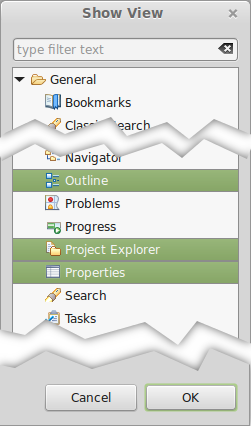
\includegraphics[width=.3\textwidth]{../rmf-images/views_highlighted.png}
\caption{Views.}
\label{fig:Views}
\end{figure}

Upon opening a ReqIF Model, the editor opens providing an overview of the model.  In essence what you are seeing is the Eclipse Workbench, with several modifications.  Here you will find a quick overview of each component.  A more detailed description of the Workbench can be found in 
\eclipsehelp{org.eclipse.platform.doc.user/reference/ref-43.htm}{Eclipse's Workbench User Guide}.

A model contains any number of specifications, and the details of each specification can be inspected individually.  The windows in which all relevant information appears are called views.  At your disposal are many views with productivity, debugging, help and team resources.  We will be focusing only on the views relevant to ProR.

% -----------------------------------------------------------------------------------
\subsection{ReqIF Overview Editor}
% -----------------------------------------------------------------------------------

This figure was briefly described in the tutorial.  Here we'll go deeper in depth.

\begin{figure}[h!]
  \centering
  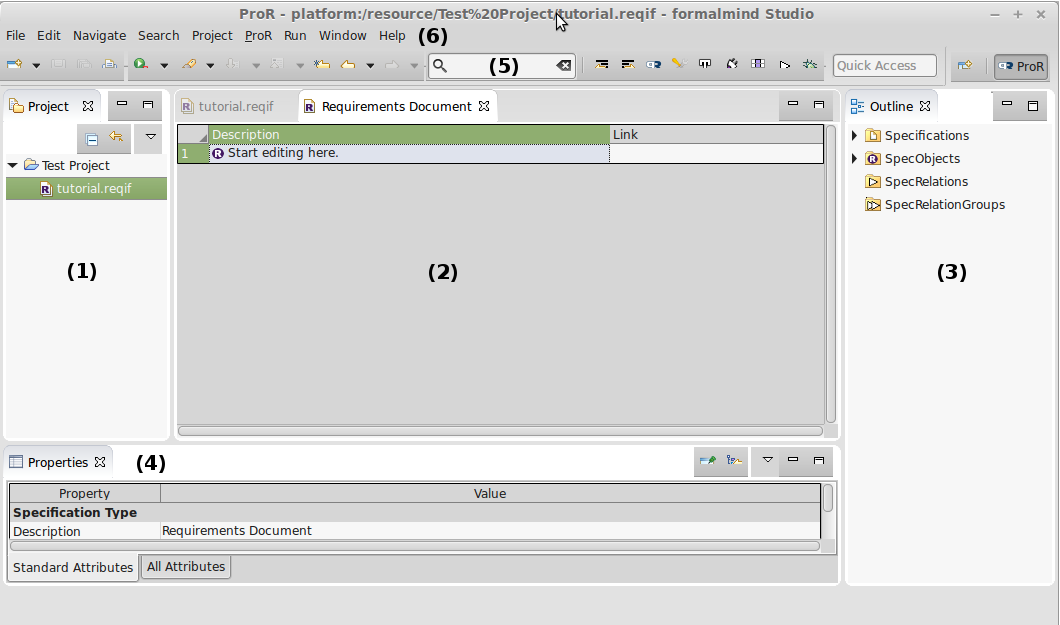
\includegraphics[width=\linewidth]{../rmf-images/Screenshot_intro.png}
  \caption{The \pror{} user interface}
  \label{fig:user_interface_overview}
\end{figure}

(1) is the Project Explorer window.  Here you will see a hierarchical listing of the project and the associated models.

(2) The Editor shows you a hierarchical breakdown of the model.  Each specification with its associated SpecObjects is listed in a spreadsheet.  Because the SpecObjects of each requirement can vary, not all fields will be completed.  Because the fields need to be created and then associated with the SpecObjects, they may not all be (nor do they need to be) represented.  But what appears and how they appear can be customized.

In the Editor, you see the SpecObjects that exist in this Specification.
There is currently only one, with the description ``Start editing here''.

The Outline (3) has four folders:

\begin{itemize}

\item
  ``Specifications'' shows the specifications in the ReqIF model.  You can
  expand the tree to expose the hierarchy of SpecObjects in the
  ReqIF model.
\item
  ``SpecObjects'' shows all SpecObjects in the ReqIF model as a flat list.
  Keep in mind that SpecObjects in Specifications are references.  In
  contrast, this folder shows all SpecObjects created for the ReqIF model, whether or not they are referenced.
\item
  ``SpecRelations'' shows all SpecRelations in the ReqIF as a flat list.
  For now, we will ignore SpecRelations.
\item
  ``SpecRelationsGroups'' represent an optional mechanism for grouping SpecRelations between two specific specifications.
\end{itemize}

The properties of a selected Element are shown in the Properties view
(4).  As the only Requirement in the model is selected, we see its
SpecObjectType (``Requirements Type'') and its only Attribute
(``Description'') with the value ``Start editing here.''.  There are two
tabs ``Standard Attributes'' and ``All Attributes'' at the bottom of the
Properties view.  \marginpar{*****} The ``Standard Attributes'' tab shows you all standard
attributes of the selected element.  The ``All Attributes'' shows all
existing ReqIF attributes of the selected element.

Above the main working windows it the tool bar (5) and, at the very top, the menu bar (6).

% -----------------------------------------------------------------------------------
\subsection{Specification Editor}
% -----------------------------------------------------------------------------------

\begin{figure}[!h]
  \centering
  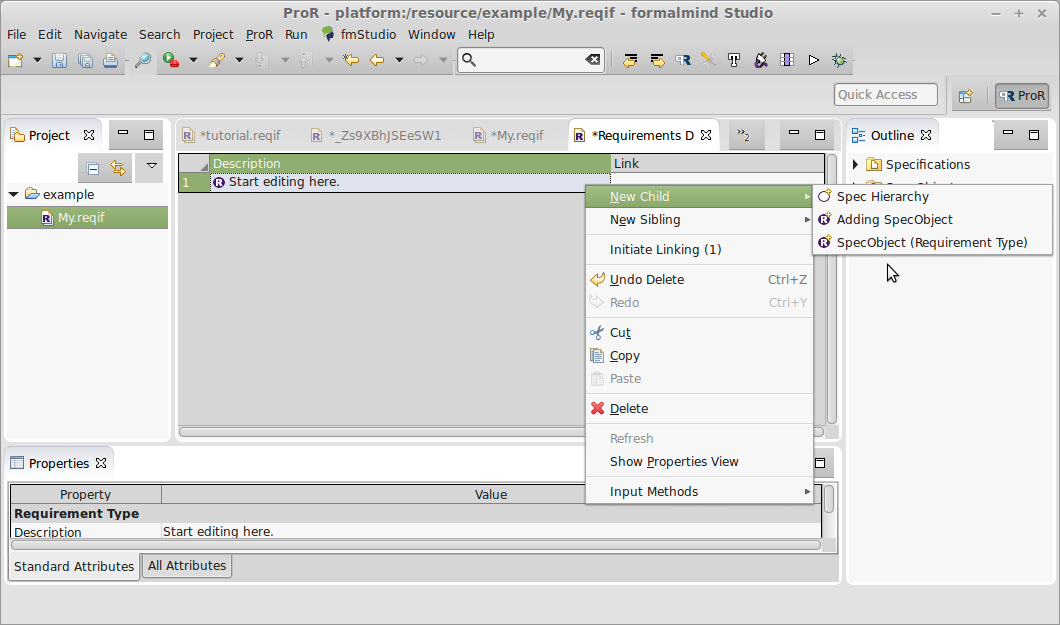
\includegraphics[width=\linewidth]{../rmf-images/default_spec_view.png}
  \caption{Default Specification Editor with the right-click menu}
  \label{fig:default specification editor}
\end{figure}
The requirements are layed out in a spreadsheet in a this window along with all their attributes in hierarchical order.

The columns, laeled across the top, display the attributes associated with each requirement. The attributes are created independantly via the Column Configurator {
\includegraphics[scale=0.6]{../rmf-images/icons/full/obj16/Column.png}. The default columns are ``Description'' and ``Link'.' ``Description`` Has two different symbols that appear on each row to the far left. Either {
\includegraphics[scale=1]{../rmf-images/icons/full/obj16/requirement.png} denoting a SpecObject (requirement). It can also display a {
\includegraphics[scale=1]{../rmf-images/icons/full/obj16/spechierarchy.png} denoting a Spec Hierarchy. 

\begin{info}
Would you like to rearrange the columns?

In the top half of the Column Configurator {
\includegraphics[scale=0.6]{../rmf-images/icons/full/obj16/Column.png}} window, a list of the exiting columns appear. Simply drag and drop them into the desired order. The changes appear in real time in the Specification Editor. Close the window and the changes will be accepted.
\end{info}

Information can be entered either directly into the cell by double clicking it or by opening the Properties Editor by right clicking any of the cells in the row. All of the SpecObjects information will then be available for editing in the Properties Editor.

The order of the rows display the hierarchy. The order in which the requirements are displayed can be easily manipulated by cutting and pasting or by dragging and dropping. To move an existing requirement into the position of parent or child of another existing requirement, simply drag the child directly \textit{onto the target parent}. Alternatively, as you drag the requirement \textit{onto the line below} the level you would like to move it, it will become a sibling rather than a child of the requirement above the line.

To duplicate a requirement, simply copy and paste it into the required position. The copying, cutting and pasting functions are accessible through the traditional dropdown menu or by right-clicking on a desired cell.

\begin{figure}[!h]
  \centering
  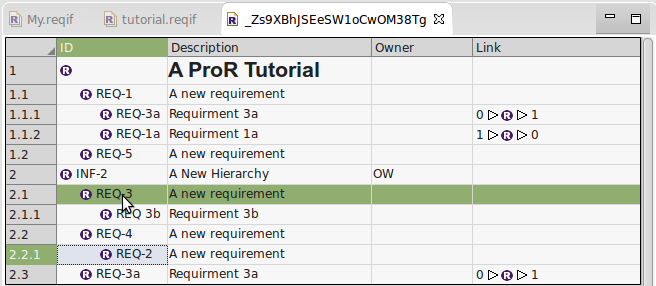
\includegraphics[width=\linewidth]{../rmf-images/hierarchy_step_1.png}
  \caption{Click on a requirement and drag onto target parent.}
  \label{fig:hierarchy_step_1}
\end{figure}
\begin{figure}[!h]
  \centering
  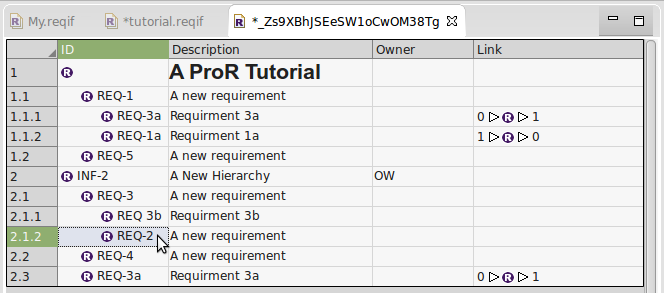
\includegraphics[width=\linewidth]{../rmf-images/hierarchy_step_2.png}
  \caption{Result: The requirement is now a child of the chosen parent.}
  \label{fig:hierarchy_step_2}
\end{figure}
\begin{figure}[!h]
  \centering
  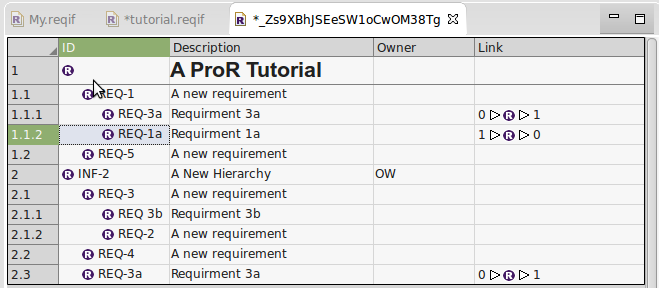
\includegraphics[width=\linewidth]{../rmf-images/hierarchy_step_3.png}
  \caption{Click on a requirement and drag onto the line (bolded) below or above target sibling.}
  \label{fig:hierarchy_step_3}
\end{figure}
\begin{figure}[!h]
  \centering
  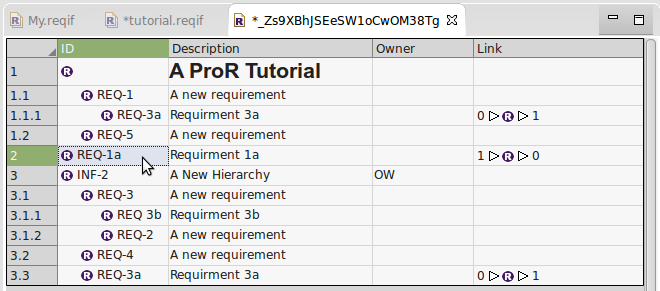
\includegraphics[width=\linewidth]{../rmf-images/hierarchy_step_4.png}
  \caption{Result: The requirement is now a sibling of the chosen requirement.}
  \label{fig:hierarchy_step_1}
\end{figure}

By right clicking on any cell in the window, you have a few options at your disposal. Outside of the usual ``Undo,'' ``Cut,'' ``Copy,'' ``Paste'' and ``Delete,'' commands, the following are also available:

\begin{description}

\item
  [New Child] - A new requirement can be created as a child of right-clicked requirement.
\item
  [New Sibling] - A new Sibling can be created on the same lever as the right-clicked requirement.
\item
  [Initiate Linking] - This is the option to create a link between requirements. Once a link is initiated and then by right clicking a target selection, the options to complete the links either to or from a selection will appear. By default, the links are illustrated in the ``Link'' column to the right. 
\item
  [Show Properties View] - Opens the Properties Editor below (be default) where one can individually inspect and edit each requirment.
\end{description}


% ===================================================================================
\section{Views}
% ===================================================================================

By default, ProR's Workbench displays the following three views:
\begin{itemize}
\item Project Explorer View: Appears on the left side and displays and allows control of the project and all it's related files.
\item Properties View: Appears at the bottom. Displays and allows the editing of highlighted objects such as projects, files, requirements, etc.
\item Outline View: Displays the structure and contents of the specifications document.
\end{itemize}

% -----------------------------------------------------------------------------------
\subsection{Project Explorer View}\index{Project Explorer View}
% -----------------------------------------------------------------------------------

TBD

% -----------------------------------------------------------------------------------
\subsection{Properties View}\index{Properties View}
% -----------------------------------------------------------------------------------

TBD

% -----------------------------------------------------------------------------------
\subsection{Outline View}\index{Outline View}
% -----------------------------------------------------------------------------------

TBD

% ===================================================================================
\section{Configurations}
% ===================================================================================

The ProR menu contains entries to launch a number of configuration
dialogs.

% -----------------------------------------------------------------------------------
\subsection{General Configuration}
\index{Configuration!General}
\label{sec:general_configuration}
% -----------------------------------------------------------------------------------

This configuration is accessed either via \menu{ProR | General Configuration}, or
via the 
\includegraphics[height=0.8em]{../rmf-images/ReqIFUIToolExtension.png} button on the toolbar.

Currently, there is only one configuration element: \menu{Label Configuration}.

\subsubsection{Label Configuration}

The ``Label Configuration'' is used to determine what to use for the text labels of elements
in places, where a shorthand is needed.  Examples are elements in the Outline or link targets.

\pror{} will determine the label by looking at the label configuration, which is a list of Strings.
It will go through the list, top to bottom.  If the element has an attribute with a matching name,
that attribute value is used as the label.

If none is found, then the element's internal ID is displayed.

To configure, select \menu{Label Configuration} in the top pane of the dialog.  On the bottom pane,
you see the \menu{Default Label} property.  Doubleclick the value (on the right), then click on the
ellipses (...) to open the configuration dialog.  Under \menu{Feature}, you see the list of attribute
names that will be used for the label, if found.

Use the \menu{Add} and \menu{Remove} buttons to add more attribute names to be searched for.  The
search order can be adjusted with \menu{Up} and \menu{Down}.

\begin{info}
It is good practice to use the ID Presentation (\ref{sec:id_presentation}) to generate
user-friendly IDs, and to use these as the first match for a label.  As IDs are unique, you'll always
have a unique identifier that is typically also used for communication.
\end{info}

% -----------------------------------------------------------------------------------
\subsection{Datatype Configuration}
\index{Configuration!Datatype}
\label{sec:datatype_configuration}
% -----------------------------------------------------------------------------------

This configuration is opened via ProR \textbar{} Datatype Configuration
...

The dialog shows two folders, one for SpecTypes and one for Datatypes.
SpecTypes are created for typing elements that have attributes
(SpecObjects, Specifications, SpecRelations).  New SpecTypes can be
created by right-clicking on the folder and selecting ``New Child''.
Through the same mechanism, attribute definitions can be added to a
SpecType.  attribute definitions are typed.  Selecting an element shows
its properties in the lower pane, where it can be configured.

Attribute definitions must have a name and a datatype.  Some attribute
definitions allow further customization.  The datatype is selected from a
dropdown.  New datatypes can be created by right-clicking on the folder
``Datatypes'' and selecting ``New Child''.  Again, selecting a datatype
shows its properties in the lower pane, where it can be configured.  A
datatype should have at least a long name.

As an example, consider the following Datatype Configuration Dialog:

\begin{figure}[h!]
\centering     
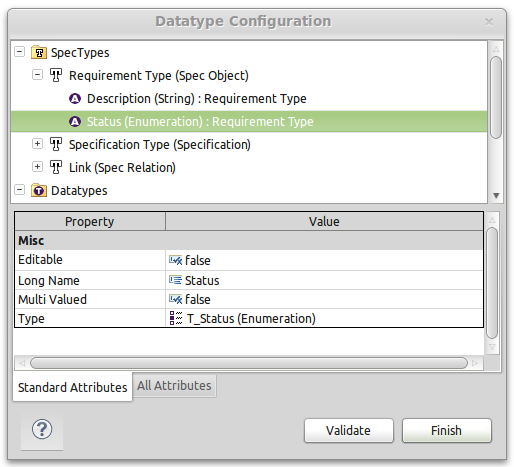
\includegraphics[width=0.8\linewidth]{../rmf-images/pror_datatype_configuration.png}
\caption{Datatype Configuration Dialog}      
\label{fig:DatatypeConfig}
\end{figure}

The Spec Type for ``Requirements Type'', which is applicable to
SpecObjects, is expanded.  The Spec Type has two attributes,
``Description'' (String) and ``Status'' (Enumeration).  Status is
selected, and in the pane below the mandatory values, ``Long Name'' and
``Type'' have been set.  Further customization of the attribute is
possible, e.g.  by converting it in a Multi-Valued attribute by setting
the corresponding flag to ``true''.

\subsubsection{Enumeration Datatypes}

An enumeration datatype must have enumeration values.  These are created
by right-clicking the enumeration datatype and selecting New Child
\textbar{} Enum Value.  You may have to unfold the enum value to select
it, so that you can provide it with a Long Name.  The following shows a
correctly configured enumeration datatype:

\begin{figure}[h!]
\centering      
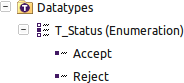
\includegraphics[width=0.4\linewidth]{../rmf-images/rmf_enumeration.png}
\caption{Enumerations}      
\label{fig:Enumerations}
\end{figure}

% -----------------------------------------------------------------------------------
\subsection{Presentation Configuration}\index{Configuration!Presentation}
\label{sec:presentation_configuration}
% -----------------------------------------------------------------------------------

% -----------------------------------------------------------------------------------
\subsection{Column Configuration}\index{Configuration!Column}
\label{sec:column_configuration}
% -----------------------------------------------------------------------------------

This configuration is specific to the Specification Editor.

The Column Configuration Dialog configures the Columns of a
Specification.  Columns are identified by name.  The width of the column
can be adjusted directly by dragging the column separator in the table
header.

If the SpecObject has an attribute where the name of the attribute
matches the name of the column, then that attribute is shown in that
column.

% ===================================================================================
\section{Elements with Values}
% ===================================================================================

TODO: Common properties of SpecObjects, SpecRelations and Specifications / Interplay between SpecType and Element / Default Values / What happens when Values are removed / How the label is determined / What Types exist / Handling of embedded objects.

% ===================================================================================
\section{SpecObjects}
% ===================================================================================

Concept of unreferenced SpecObjects in the Outline and referenced SpecObjects from Specifications.

% ===================================================================================
\section{Specifications}
% ===================================================================================

Container for SpecHierarchies / Referencing SpecObjects / TableInternal feature

% ===================================================================================
\section{SpecRelations}
% ===================================================================================

Navigating Source and Target / Representation in Specification Editor / Linking across ReqIF models.

% ===================================================================================
\section{SpecRelationGroups}
% ===================================================================================

History / Limitations due to bug in Schema.

% ===================================================================================
\section{Access Control}
% ===================================================================================



% ===================================================================================
\section{Import and Export}
% ===================================================================================

% ===================================================================================
\section{Searching and Filtering}
% ===================================================================================

